% SSU Data Dash 2026: team report. Compile from this folder (Overleaf: upload the whole
% repository as a zip). `python run.py report` and `python run.py analysis` write the table and figures.
\documentclass[11pt]{article}
\usepackage[margin=2.2cm]{geometry}
\usepackage{graphicx,booktabs,hyperref}
\graphicspath{{../figures/}}
\setlength{\parskip}{4pt}

\title{SSU Data Dash 2026: \textit{What is this home worth today?}\\[2pt]\large Team YOUR TEAM NAME}
\author{First Last, First Last, First Last}
\date{}

\begin{document}
\maketitle

\noindent\begin{tabular}{@{}ll}
\textbf{Video (YouTube):} & \url{https://youtu.be/YOUR-VIDEO} \\
\textbf{Code and submission files (GitHub):} & \url{https://github.com/YOUR-NAME/SSU-Data-Dash} \\
\end{tabular}

\section*{Summary}
The starter values an off-market home as the median of the ten nearest past sales. That fails
for three reasons: the sales are from a different market (2022 vs 2026), they are different
sizes, and nothing about the home itself is used. We fix each of these. A \textbf{market index}
converts every past sale to today's dollars. \textbf{Leak-free comparable-sales and neighbourhood
features} describe location in those dollars, and listing-text flags describe condition. A
gradient-boosted model learns the rest. On walk-forward validation (December 2025 to May 2026)
the off-market MdAPE falls from 20.8\% to \textbf{7.86\%}, and the list-aware MdAPE from 7.3\%
to \textbf{3.96\%}. The main lesson: \emph{time} is the biggest error source. That holds
for price levels and also for sold-to-list ratios, which drifted as bidding wars faded.

\section{Data and features}
All features come from columns available in the test files. Anything known only after the sale
(sold price, sale date, days on market, the third-party estimate) is never used. Every learned
quantity is computed inside \texttt{FeatureBuilder.fit()} from the training sales only.
\begin{itemize}\itemsep0pt
\item \textbf{Market index.} For each property type and month, the median residual log price
after removing each sale's community-by-type level (two passes), smoothed over 3 months. Prices
are converted to last-month dollars, and test homes are priced at the latest level.
\item \textbf{Comparable sales.} The 10 nearest past sales of the same type (KD-tree on
latitude/longitude): median adjusted price, price per sq ft, nearest-3 median, distance to the
10th comparable. A training home never counts itself.
\item \textbf{Neighbourhood levels.} Adjusted price per sq ft by community and by
community$\times$type, shrunk toward the type mean (20-sale prior). Training rows get
5-fold out-of-fold values to avoid target leakage.
\item \textbf{Home and text.} Square feet (range midpoints), rooms, parking, garage, lot size,
style, municipality, coordinates, listing month, and nine keyword groups from the remarks
(renovated, needs work/as-is, luxury, views/ravine, pool, basement/income suite, transit,
corner, penthouse).
\item \textbf{List-aware only.} Log list price, list price in today's dollars, list price minus
comparable value, list price minus neighbourhood value, round-number and \$\ldots9,000 pricing flags.
\end{itemize}

\section{Models}
\textbf{Off-market.} Histogram gradient boosting (600 trees, 63 leaves, learning rate 0.05) on log
price in today's dollars. The list price is removed before the model sees the homes.

\textbf{List-aware.} The same learner predicts the \emph{log sold-to-list ratio}, which is then
multiplied by the list price. The list price already carries most of the information, so the
model only learns the gap. Our first version learned one ratio level from all five years and
predicted 2.4\% too high in \emph{every} validation month: the 2022 over-asking market had
faded. We added a \emph{ratio index} (median log ratio per type and month). The model learns each
sale's ratio relative to its month, and test homes get the median ratio of the last three
training months. This was the only change we made after seeing validation results, and we
report both versions.

\textbf{Uncertainty.} Two quantile models (10th and 90th percentile) give an 80\% price range
for every home.

\section{Validation}
We used the starter's walk-forward scheme: for each month from December 2025 to May 2026, all
models are retrained from scratch on sales strictly before that month and predict that month's
homes, with answer columns removed by \texttt{data.hide\_answers}. No random split and no tuning
loop on these months. Hyper-parameters are fixed, sensible defaults. Unit tests check that the
baseline never uses later sales and that the full pipeline runs end to end.

\section{Results}
\begin{table}[h]
\centering
\small
% Written by `python run.py report`. Do not edit by hand: rerun the command instead.
\begin{tabular}{lrccc}
\hline
Track & Homes & MdAPE \% (95\% CI) & MAPE \% (95\% CI) & Median signed error \% \\
\hline
off-market & 10,069 & 6.96 (6.82--7.11) & 9.25 (9.06--9.43) & +0.80 \\
list-aware & 10,069 & 3.96 (3.87--4.06) & 5.04 (4.96--5.12) & +0.83 \\
\hline
\end{tabular}

\caption{Walk-forward validation, Dec 2025 to May 2026 (10,069 homes per track). Brackets:
bootstrap 95\% interval.}
\end{table}

\begin{table}[h]
\centering
\small
\begin{tabular}{llcc}
\toprule
Track & Model & MdAPE & MAPE \\
\midrule
Both & Maximum error (type $\times$ community 12-month median) & 17.7\% & 22.0\% \\
Off-market & Starter: 10 nearest earlier sales & 20.8\% & 27.4\% \\
Off-market & \textbf{Ours} & \textbf{7.86\%} & \textbf{10.18\%} \\
List-aware & Starter: list price & 7.3\% & 8.1\% \\
List-aware & Ours, first version (no ratio index) & 4.53\% & 5.68\% \\
List-aware & \textbf{Ours, final} & \textbf{3.96\%} & \textbf{5.11\%} \\
\bottomrule
\end{tabular}
\caption{Against the baselines (baseline figures from the case handout).}
\end{table}

Off-market error falls by 62\% against the starter and is well under the 17.7\% bar. The error
is stable from month to month (7.4\% to 8.0\%), which suggests the hidden test will land nearby.
The off-market median signed error is $-0.35\%$, so there is no systematic bias. Our 80\% ranges
held the sold price 73.9\% (off-market) and 78.9\% (list-aware) of the time, slightly below
80\%. The off-market ranges are a little too narrow and should be widened about 10\% before being relied on.

\section{Where the model fails}
\begin{figure}[h]
\centering
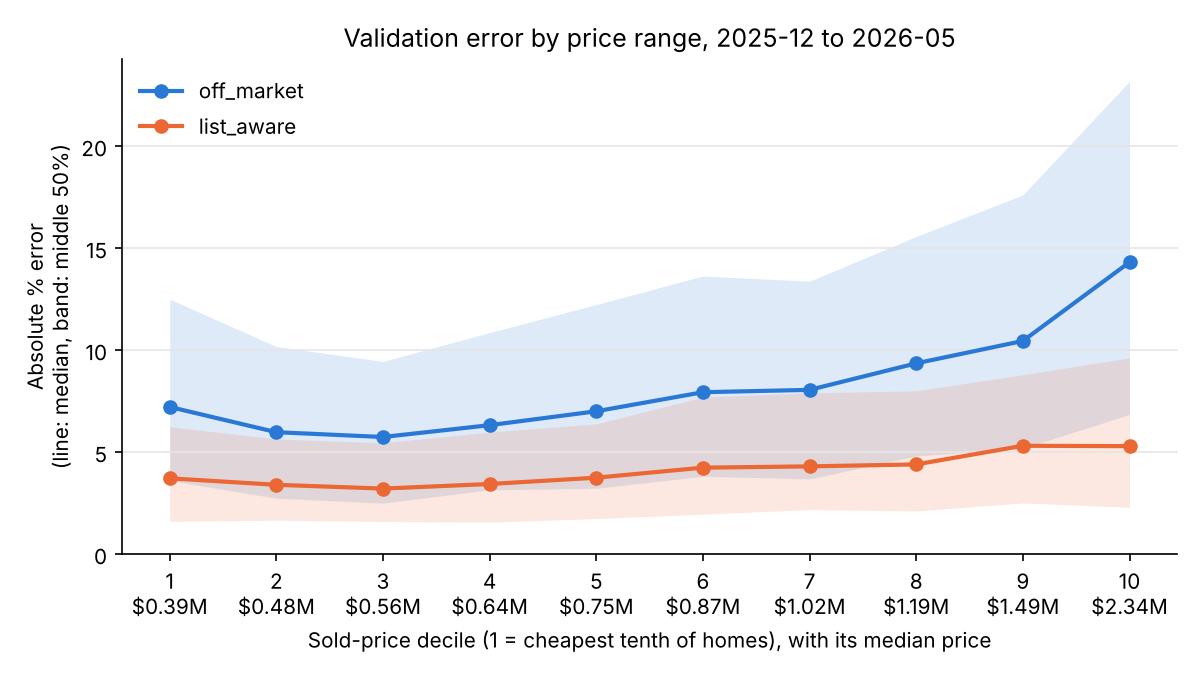
\includegraphics[width=0.49\linewidth]{error_by_price_range.png}
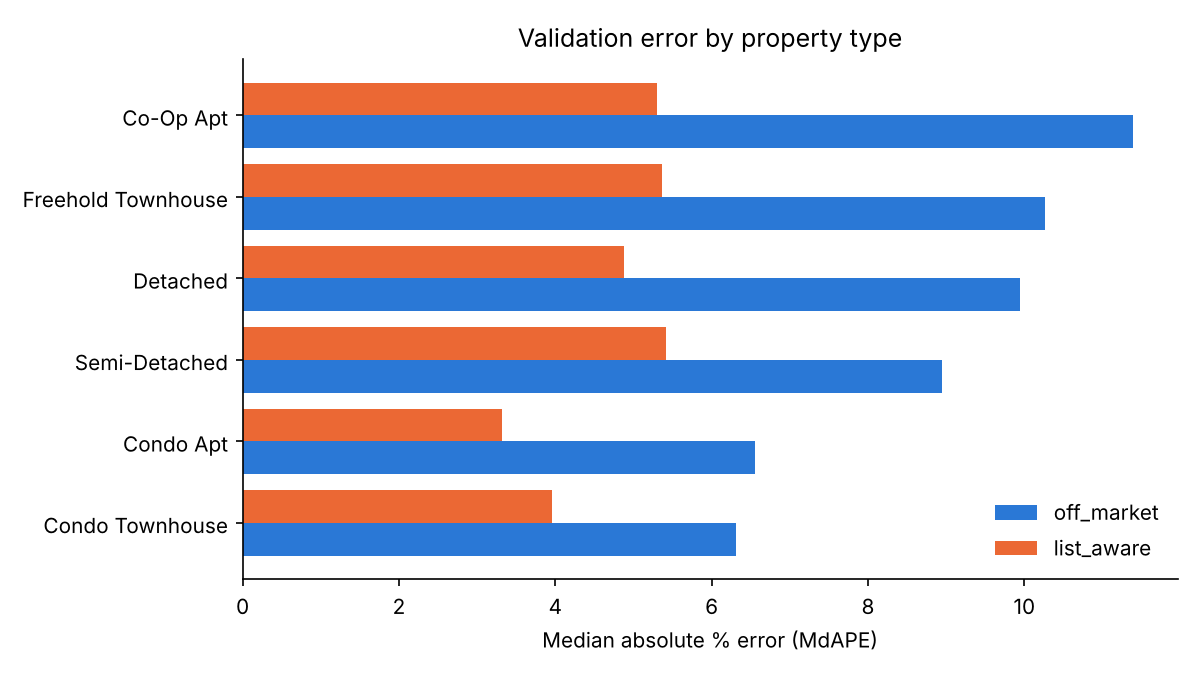
\includegraphics[width=0.49\linewidth]{error_by_type.png}
\caption{Absolute \% error by sold-price decile (left) and by property type (right).}
\end{figure}
\textbf{By type.} Condos are easiest off-market (6.6\% MdAPE): units in one building share a
location and comparables. Detached homes (9.9\%), freehold townhouses (10.3\%) and especially
co-ops (11.4\%, only 48 homes, MAPE 19\%) are hardest. For freehold homes, lot, layout and
condition vary far more than our features capture.
\textbf{By neighbourhood.} The worst communities (e.g.\ Maplepark, Hazelfield: 15--16\% MdAPE)
have large \emph{signed} errors ($-5\%$ to $-11\%$). We under-predict them consistently, which
suggests their prices are moving faster than the type-level market index. A community-level
index would be the next step.
\textbf{By price.} Errors are highest at the extremes, where comparables are scarce and the
model pulls toward typical prices.
\textbf{By month.} Off-market bias swings between $-2.7\%$ and $+3.0\%$ month to month. This is
market noise no model can foresee.

\section{Limitations}
The hidden test is 1--4 months past the last training sale, while validation is always 1 month
ahead. If prices move over the summer, our flat index will miss it, so hidden-test error may be
somewhat higher. The 80\% ranges under-cover. Text features are simple keyword flags; a sentence
embedding of the remarks could capture condition better. Do not trust the model for co-ops,
for the top and bottom price deciles, or in communities with few recent sales.

\section*{Outside data}
\begin{tabular}{lll}
\toprule
Source & URL & Periods covered \\
\midrule
None & --- & --- \\
\bottomrule
\end{tabular}

\section*{Reproducing our results}
\texttt{pip install -r requirements.txt}\\
\texttt{python run.py validate \&\& python run.py report \&\& python run.py analysis}\\
\texttt{python run.py predict \&\& python run.py check}

\end{document}
